\subsection{SCV Units}

The \textit{Terran} race uses SCV units to harvest resources and build structures. At the start of a game there are four SCVs available to the player.

Figure~\ref{fig:scv_diagram} shows the Markov Chain which dictates the behaviour of the SCV units. The transition from Building to Idle has no probability assigned to it. Building is taken to be a distinct state but exiting the state is controlled by the game, not the agent. The probabilities \(P_{IB}\) and \(P_{IH}\) refer to the probability that an idle agent will chose to start harvesting or to start building. \(P_{HB}\) refers to the probability of a harvesting agent stopping and beginning building.

\begin{figure}
\centering
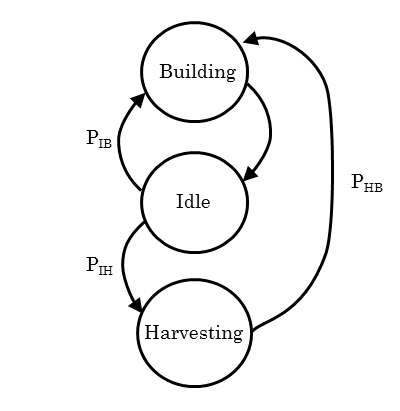
\includegraphics[scale=0.8, trim = 0cm 0cm 0cm 0cm]{diagrams/scv}
\label{fig:scv_diagram}
\caption{Markov Chain for SCV agent.}
\end{figure}